% Options for packages loaded elsewhere
\PassOptionsToPackage{unicode}{hyperref}
\PassOptionsToPackage{hyphens}{url}
%
\documentclass[
]{article}
\usepackage{amsmath,amssymb}
\usepackage{iftex}
\ifPDFTeX
  \usepackage[T1]{fontenc}
  \usepackage[utf8]{inputenc}
  \usepackage{textcomp} % provide euro and other symbols
\else % if luatex or xetex
  \usepackage{unicode-math} % this also loads fontspec
  \defaultfontfeatures{Scale=MatchLowercase}
  \defaultfontfeatures[\rmfamily]{Ligatures=TeX,Scale=1}
\fi
\usepackage{lmodern}
\ifPDFTeX\else
  % xetex/luatex font selection
\fi
% Use upquote if available, for straight quotes in verbatim environments
\IfFileExists{upquote.sty}{\usepackage{upquote}}{}
\IfFileExists{microtype.sty}{% use microtype if available
  \usepackage[]{microtype}
  \UseMicrotypeSet[protrusion]{basicmath} % disable protrusion for tt fonts
}{}
\makeatletter
\@ifundefined{KOMAClassName}{% if non-KOMA class
  \IfFileExists{parskip.sty}{%
    \usepackage{parskip}
  }{% else
    \setlength{\parindent}{0pt}
    \setlength{\parskip}{6pt plus 2pt minus 1pt}}
}{% if KOMA class
  \KOMAoptions{parskip=half}}
\makeatother
\usepackage{xcolor}
\usepackage[margin=1in]{geometry}
\usepackage{color}
\usepackage{fancyvrb}
\newcommand{\VerbBar}{|}
\newcommand{\VERB}{\Verb[commandchars=\\\{\}]}
\DefineVerbatimEnvironment{Highlighting}{Verbatim}{commandchars=\\\{\}}
% Add ',fontsize=\small' for more characters per line
\usepackage{framed}
\definecolor{shadecolor}{RGB}{248,248,248}
\newenvironment{Shaded}{\begin{snugshade}}{\end{snugshade}}
\newcommand{\AlertTok}[1]{\textcolor[rgb]{0.94,0.16,0.16}{#1}}
\newcommand{\AnnotationTok}[1]{\textcolor[rgb]{0.56,0.35,0.01}{\textbf{\textit{#1}}}}
\newcommand{\AttributeTok}[1]{\textcolor[rgb]{0.13,0.29,0.53}{#1}}
\newcommand{\BaseNTok}[1]{\textcolor[rgb]{0.00,0.00,0.81}{#1}}
\newcommand{\BuiltInTok}[1]{#1}
\newcommand{\CharTok}[1]{\textcolor[rgb]{0.31,0.60,0.02}{#1}}
\newcommand{\CommentTok}[1]{\textcolor[rgb]{0.56,0.35,0.01}{\textit{#1}}}
\newcommand{\CommentVarTok}[1]{\textcolor[rgb]{0.56,0.35,0.01}{\textbf{\textit{#1}}}}
\newcommand{\ConstantTok}[1]{\textcolor[rgb]{0.56,0.35,0.01}{#1}}
\newcommand{\ControlFlowTok}[1]{\textcolor[rgb]{0.13,0.29,0.53}{\textbf{#1}}}
\newcommand{\DataTypeTok}[1]{\textcolor[rgb]{0.13,0.29,0.53}{#1}}
\newcommand{\DecValTok}[1]{\textcolor[rgb]{0.00,0.00,0.81}{#1}}
\newcommand{\DocumentationTok}[1]{\textcolor[rgb]{0.56,0.35,0.01}{\textbf{\textit{#1}}}}
\newcommand{\ErrorTok}[1]{\textcolor[rgb]{0.64,0.00,0.00}{\textbf{#1}}}
\newcommand{\ExtensionTok}[1]{#1}
\newcommand{\FloatTok}[1]{\textcolor[rgb]{0.00,0.00,0.81}{#1}}
\newcommand{\FunctionTok}[1]{\textcolor[rgb]{0.13,0.29,0.53}{\textbf{#1}}}
\newcommand{\ImportTok}[1]{#1}
\newcommand{\InformationTok}[1]{\textcolor[rgb]{0.56,0.35,0.01}{\textbf{\textit{#1}}}}
\newcommand{\KeywordTok}[1]{\textcolor[rgb]{0.13,0.29,0.53}{\textbf{#1}}}
\newcommand{\NormalTok}[1]{#1}
\newcommand{\OperatorTok}[1]{\textcolor[rgb]{0.81,0.36,0.00}{\textbf{#1}}}
\newcommand{\OtherTok}[1]{\textcolor[rgb]{0.56,0.35,0.01}{#1}}
\newcommand{\PreprocessorTok}[1]{\textcolor[rgb]{0.56,0.35,0.01}{\textit{#1}}}
\newcommand{\RegionMarkerTok}[1]{#1}
\newcommand{\SpecialCharTok}[1]{\textcolor[rgb]{0.81,0.36,0.00}{\textbf{#1}}}
\newcommand{\SpecialStringTok}[1]{\textcolor[rgb]{0.31,0.60,0.02}{#1}}
\newcommand{\StringTok}[1]{\textcolor[rgb]{0.31,0.60,0.02}{#1}}
\newcommand{\VariableTok}[1]{\textcolor[rgb]{0.00,0.00,0.00}{#1}}
\newcommand{\VerbatimStringTok}[1]{\textcolor[rgb]{0.31,0.60,0.02}{#1}}
\newcommand{\WarningTok}[1]{\textcolor[rgb]{0.56,0.35,0.01}{\textbf{\textit{#1}}}}
\usepackage{graphicx}
\makeatletter
\def\maxwidth{\ifdim\Gin@nat@width>\linewidth\linewidth\else\Gin@nat@width\fi}
\def\maxheight{\ifdim\Gin@nat@height>\textheight\textheight\else\Gin@nat@height\fi}
\makeatother
% Scale images if necessary, so that they will not overflow the page
% margins by default, and it is still possible to overwrite the defaults
% using explicit options in \includegraphics[width, height, ...]{}
\setkeys{Gin}{width=\maxwidth,height=\maxheight,keepaspectratio}
% Set default figure placement to htbp
\makeatletter
\def\fps@figure{htbp}
\makeatother
\setlength{\emergencystretch}{3em} % prevent overfull lines
\providecommand{\tightlist}{%
  \setlength{\itemsep}{0pt}\setlength{\parskip}{0pt}}
\setcounter{secnumdepth}{-\maxdimen} % remove section numbering
\ifLuaTeX
  \usepackage{selnolig}  % disable illegal ligatures
\fi
\usepackage{bookmark}
\IfFileExists{xurl.sty}{\usepackage{xurl}}{} % add URL line breaks if available
\urlstyle{same}
\hypersetup{
  pdftitle={Supervised Learning},
  hidelinks,
  pdfcreator={LaTeX via pandoc}}

\title{Supervised Learning}
\author{}
\date{\vspace{-2.5em}06/01/2025}

\begin{document}
\maketitle

\section{Detección de ataques con aprendizaje
supervisado}\label{detecciuxf3n-de-ataques-con-aprendizaje-supervisado}

El siguiente ejercicio consiste en la optmización de un modelo de
Machine Learning capaz de detectar ataques a partir de logs de un
firewall. Para este propósito, se realizará una prueba de concepto con
una pequeña muestra de logs previamente etiquetados como tráfico normal
o ataque.

\subsection{Load of the data sets}\label{load-of-the-data-sets}

Se proporcionan los siguentes archivos:

\begin{itemize}
\tightlist
\item
  features.csv
\item
  events.csv
\end{itemize}

\subsubsection{Events
analysis/exploration}\label{events-analysisexploration}

\subsubsection{Data enrichment}\label{data-enrichment}

\begin{verbatim}
##     srcip               sport          dstip               dsport     
##  Length:10000       Min.   :    0   Length:10000       Min.   :    0  
##  Class :character   1st Qu.:10325   Class :character   1st Qu.:   53  
##  Mode  :character   Median :31422   Mode  :character   Median :   80  
##                     Mean   :30269                      Mean   :10944  
##                     3rd Qu.:47439                      3rd Qu.:13531  
##                     Max.   :65535                      Max.   :65535  
##                                                                       
##     proto              state                dur               sbytes       
##  Length:10000       Length:10000       Min.   : 0.00000   Min.   :     46  
##  Class :character   Class :character   1st Qu.: 0.00104   1st Qu.:    264  
##  Mode  :character   Mode  :character   Median : 0.01585   Median :   1540  
##                                        Mean   : 0.66818   Mean   :   4418  
##                                        3rd Qu.: 0.22312   3rd Qu.:   3182  
##                                        Max.   :59.99847   Max.   :5127548  
##                                                                            
##      dbytes             sttl             dttl            sloss         
##  Min.   :      0   Min.   :  0.00   Min.   :  0.00   Min.   :   0.000  
##  1st Qu.:    164   1st Qu.: 31.00   1st Qu.: 29.00   1st Qu.:   0.000  
##  Median :   1888   Median : 31.00   Median : 29.00   Median :   3.000  
##  Mean   :  38307   Mean   : 62.57   Mean   : 30.59   Mean   :   5.316  
##  3rd Qu.:  15036   3rd Qu.: 31.00   3rd Qu.: 29.00   3rd Qu.:   7.000  
##  Max.   :2389599   Max.   :254.00   Max.   :252.00   Max.   :1906.000  
##                                                                        
##      dloss          service              Sload               Dload         
##  Min.   :  0.00   Length:10000       Min.   :0.000e+00   Min.   :       0  
##  1st Qu.:  0.00   Class :character   1st Qu.:1.237e+05   1st Qu.:    9625  
##  Median :  4.00   Mode  :character   Median :5.977e+05   Median :  589668  
##  Mean   : 17.06                      Mean   :3.899e+07   Mean   : 2464173  
##  3rd Qu.: 14.00                      3rd Qu.:2.266e+06   3rd Qu.: 3027574  
##  Max.   :856.00                      Max.   :5.268e+09   Max.   :20439672  
##                                                                            
##      Spkts             Dpkts              swin            dwin      
##  Min.   :   1.00   Min.   :   0.00   Min.   :  0.0   Min.   :  0.0  
##  1st Qu.:   2.00   1st Qu.:   2.00   1st Qu.:  0.0   1st Qu.:  0.0  
##  Median :  12.00   Median :  12.00   Median :255.0   Median :255.0  
##  Mean   :  34.28   Mean   :  44.41   Mean   :151.1   Mean   :150.6  
##  3rd Qu.:  44.00   3rd Qu.:  42.00   3rd Qu.:255.0   3rd Qu.:255.0  
##  Max.   :3818.00   Max.   :1716.00   Max.   :255.0   Max.   :255.0  
##                                                                     
##      stcpb               dtcpb              smeansz          dmeansz      
##  Min.   :0.000e+00   Min.   :0.000e+00   Min.   :  28.0   Min.   :   0.0  
##  1st Qu.:0.000e+00   1st Qu.:0.000e+00   1st Qu.:  61.0   1st Qu.:  69.0  
##  Median :6.558e+08   Median :6.364e+08   Median :  73.0   Median :  89.0  
##  Mean   :1.268e+09   Mean   :1.272e+09   Mean   : 123.1   Mean   : 278.4  
##  3rd Qu.:2.479e+09   3rd Qu.:2.508e+09   3rd Qu.: 132.0   3rd Qu.: 565.0  
##  Max.   :4.294e+09   Max.   :4.295e+09   Max.   :1500.0   Max.   :1465.0  
##                                                                           
##   trans_depth      res_bdy_len           Sjit               Djit         
##  Min.   :0.0000   Min.   :      0   Min.   :     0.0   Min.   :    0.00  
##  1st Qu.:0.0000   1st Qu.:      0   1st Qu.:     0.0   1st Qu.:    0.00  
##  Median :0.0000   Median :      0   Median :    18.9   Median :    2.65  
##  Mean   :0.0855   Mean   :   4688   Mean   :  1783.8   Mean   :  741.70  
##  3rd Qu.:0.0000   3rd Qu.:      0   3rd Qu.:   425.9   3rd Qu.:   64.66  
##  Max.   :2.0000   Max.   :1159260   Max.   :957257.4   Max.   :37907.53  
##                                                                          
##      Stime               Ltime              Sintpkt            Dintpkt        
##  Min.   :1.422e+09   Min.   :1.422e+09   Min.   :    0.00   Min.   :    0.00  
##  1st Qu.:1.422e+09   1st Qu.:1.422e+09   1st Qu.:    0.01   1st Qu.:    0.01  
##  Median :1.424e+09   Median :1.424e+09   Median :    0.47   Median :    0.41  
##  Mean   :1.423e+09   Mean   :1.423e+09   Mean   :  237.63   Mean   :  102.28  
##  3rd Qu.:1.424e+09   3rd Qu.:1.424e+09   3rd Qu.:    7.27   3rd Qu.:    6.12  
##  Max.   :1.424e+09   Max.   :1.424e+09   Max.   :60000.83   Max.   :50103.18  
##                                                                               
##      tcprtt             synack             ackdat         is_sm_ips_ports 
##  Min.   :0.000000   Min.   :0.000000   Min.   :0.000000   Min.   :0.0000  
##  1st Qu.:0.000000   1st Qu.:0.000000   1st Qu.:0.000000   1st Qu.:0.0000  
##  Median :0.000615   Median :0.000484   Median :0.000122   Median :0.0000  
##  Mean   :0.006682   Mean   :0.003546   Mean   :0.003136   Mean   :0.0021  
##  3rd Qu.:0.000704   3rd Qu.:0.000555   3rd Qu.:0.000141   3rd Qu.:0.0000  
##  Max.   :2.099150   Max.   :1.990589   Max.   :1.186523   Max.   :1.0000  
##                                                                           
##   ct_state_ttl    ct_flw_http_mthd  is_ftp_login     ct_ftp_cmd  
##  Min.   :0.0000   Min.   : 0.000   Min.   :0.000   Min.   :0.00  
##  1st Qu.:0.0000   1st Qu.: 0.000   1st Qu.:0.000   1st Qu.:0.00  
##  Median :0.0000   Median : 0.000   Median :0.000   Median :0.00  
##  Mean   :0.2583   Mean   : 0.236   Mean   :0.035   Mean   :0.04  
##  3rd Qu.:0.0000   3rd Qu.: 0.000   3rd Qu.:0.000   3rd Qu.:0.00  
##  Max.   :6.0000   Max.   :30.000   Max.   :4.000   Max.   :5.00  
##                   NA's   :5371     NA's   :5702    NA's   :5702  
##    ct_srv_src       ct_srv_dst       ct_dst_ltm       ct_src_ltm    
##  Min.   : 1.000   Min.   : 1.000   Min.   : 1.000   Min.   : 1.000  
##  1st Qu.: 2.000   1st Qu.: 2.000   1st Qu.: 2.000   1st Qu.: 2.000  
##  Median : 5.000   Median : 5.000   Median : 3.000   Median : 4.000  
##  Mean   : 9.234   Mean   : 9.001   Mean   : 6.423   Mean   : 6.905  
##  3rd Qu.:11.000   3rd Qu.:10.000   3rd Qu.: 6.000   3rd Qu.: 7.000  
##  Max.   :63.000   Max.   :63.000   Max.   :60.000   Max.   :60.000  
##                                                                     
##  ct_src_dport_ltm ct_dst_sport_ltm ct_dst_src_ltm    attack_cat       
##  Min.   : 1.000   Min.   : 1.000   Min.   : 1.000   Length:10000      
##  1st Qu.: 1.000   1st Qu.: 1.000   1st Qu.: 1.000   Class :character  
##  Median : 1.000   Median : 1.000   Median : 2.000   Mode  :character  
##  Mean   : 4.661   Mean   : 3.603   Mean   : 6.852                     
##  3rd Qu.: 2.000   3rd Qu.: 1.000   3rd Qu.: 5.000                     
##  Max.   :60.000   Max.   :60.000   Max.   :63.000                     
##                                                                       
##      Label       
##  Min.   :0.0000  
##  1st Qu.:0.0000  
##  Median :0.0000  
##  Mean   :0.1251  
##  3rd Qu.:0.0000  
##  Max.   :1.0000  
## 
\end{verbatim}

\subsection{Feature engineering}\label{feature-engineering}

\begin{verbatim}
## 
## ATTACK NORMAL 
## 0.1251 0.8749
\end{verbatim}

\subsection{Build model}\label{build-model}

\subsubsection{Create train and test data
sets}\label{create-train-and-test-data-sets}

\subsubsection{Prepare object with training configuration (how we are
gonna train the
model)}\label{prepare-object-with-training-configuration-how-we-are-gonna-train-the-model}

\subsubsection{Train the model}\label{train-the-model}

\begin{verbatim}
## Iter   TrainDeviance   ValidDeviance   StepSize   Improve
##      1        0.5883             nan     0.1000    0.0814
##      2        0.4994             nan     0.1000    0.0411
##      3        0.4349             nan     0.1000    0.0320
##      4        0.3848             nan     0.1000    0.0248
##      5        0.3458             nan     0.1000    0.0204
##      6        0.3119             nan     0.1000    0.0167
##      7        0.2823             nan     0.1000    0.0146
##      8        0.2575             nan     0.1000    0.0115
##      9        0.2360             nan     0.1000    0.0108
##     10        0.2163             nan     0.1000    0.0095
##     20        0.1195             nan     0.1000    0.0030
##     40        0.0768             nan     0.1000   -0.0001
##     50        0.0719             nan     0.1000   -0.0002
\end{verbatim}

\subsubsection{Test model}\label{test-model}

\subsection{Evaluate model}\label{evaluate-model}

\begin{verbatim}
##  Accuracy     Kappa 
## 0.9837312 0.9277821
\end{verbatim}

\begin{Shaded}
\begin{Highlighting}[]
\CommentTok{\# probabilites}
\NormalTok{predictions }\OtherTok{\textless{}{-}} \FunctionTok{predict}\NormalTok{(}\AttributeTok{object =}\NormalTok{ objModel, testDF[,predictorsNames], }\AttributeTok{type =} \StringTok{\textquotesingle{}prob\textquotesingle{}}\NormalTok{)}
\NormalTok{auc }\OtherTok{\textless{}{-}}\NormalTok{ pROC}\SpecialCharTok{::}\FunctionTok{roc}\NormalTok{(}\FunctionTok{ifelse}\NormalTok{(testDF[,outcomeName] }\SpecialCharTok{==} \StringTok{"ATTACK"}\NormalTok{,}\DecValTok{1}\NormalTok{,}\DecValTok{0}\NormalTok{), predictions[[}\DecValTok{2}\NormalTok{]])}
\end{Highlighting}
\end{Shaded}

\begin{verbatim}
## Setting levels: control = 0, case = 1
\end{verbatim}

\begin{verbatim}
## Setting direction: controls > cases
\end{verbatim}

\begin{Shaded}
\begin{Highlighting}[]
\FunctionTok{print}\NormalTok{(auc}\SpecialCharTok{$}\NormalTok{auc)}
\end{Highlighting}
\end{Shaded}

\begin{verbatim}
## Area under the curve: 0.9978
\end{verbatim}

\begin{Shaded}
\begin{Highlighting}[]
\FunctionTok{plot}\NormalTok{(caret}\SpecialCharTok{::}\FunctionTok{varImp}\NormalTok{(objModel, }\AttributeTok{scale =}\NormalTok{ F))}
\end{Highlighting}
\end{Shaded}

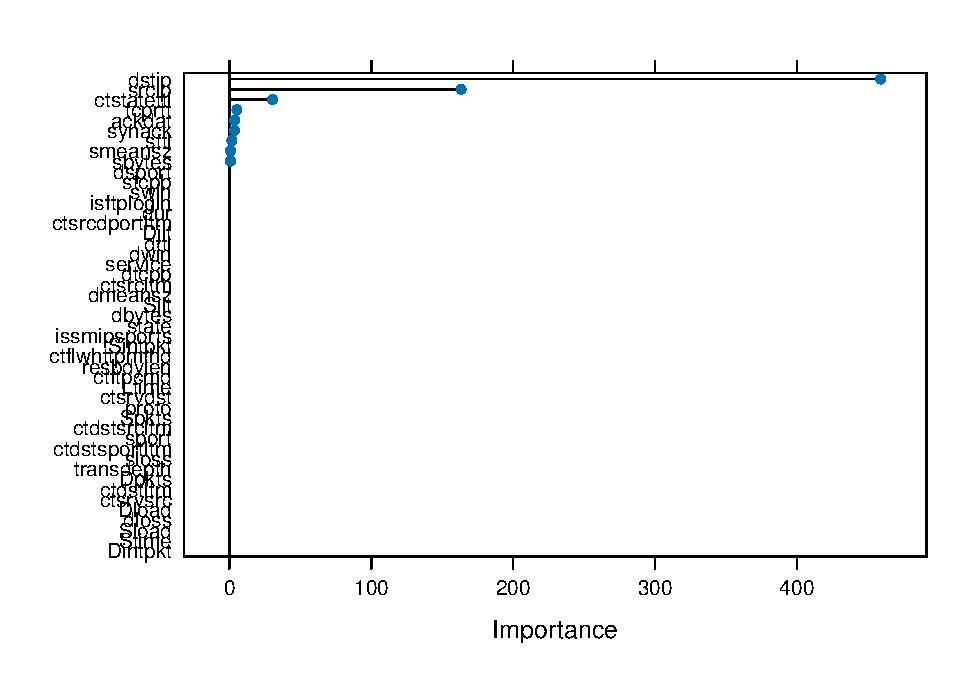
\includegraphics{supervised_files/figure-latex/var_importance-1.pdf}

\subsection{Conclusiones}\label{conclusiones}

Aqui deben incluirse los cambios hechos en el codigo que han
incrementado la precision del modelo.

\end{document}
